\chapter{Seznámení s HEAppE Middleware}
Kapitola je zaměřena na popis aplikačního rámce HEAppE Middleware.

\section{Účel HEAppE Middleware}
HEAppE Middleware (High-End Application Execution Middleware) poskytuje aplikační rozhraní (API) pro kompletní správu úlohy na superpočítačovém clusteru, od vytvoření až po přenos zpracovaných dat. Jedná se o open-source projekt implementující koncept HPC-as-a-Service a jeho cílem je zjednodušit komunikaci s HPC plánovačem a umožnit uživateli pohodlnou implementaci do jeho klientské aplikace. HEAppE Middleware zajišťuje bezpečnou a šifrovanou komunikaci s výpočetním clusterem prostřednictvím protokolu SSH. Komunikace pak stojí na autentizaci pomocí asymetrického šifrování s využitím veřejného klíče (RSA).

Abstraktně si můžeme HEAppE Middleware představit jako spolehlivého prostředníka mezi uživatelem a výpočetním clusterem, popř. jeho plánovačem. Poskytuje uživatelům vzdálený přístup k výpočetním clusterům se zaměřením na bezpečnost a jednoduchost přístupu.

Prakticky se jedná o službu, prostřednictvím které může koncový uživatel komunikovat s HPC clusterem přes standardizované aplikační rozhraní zvané jako REST API, stojící na HTTP komunikaci.

Následuje ilustrace popisující využití HPC-as-a-Service / HaaS.

\begin{figure}
	\centering
	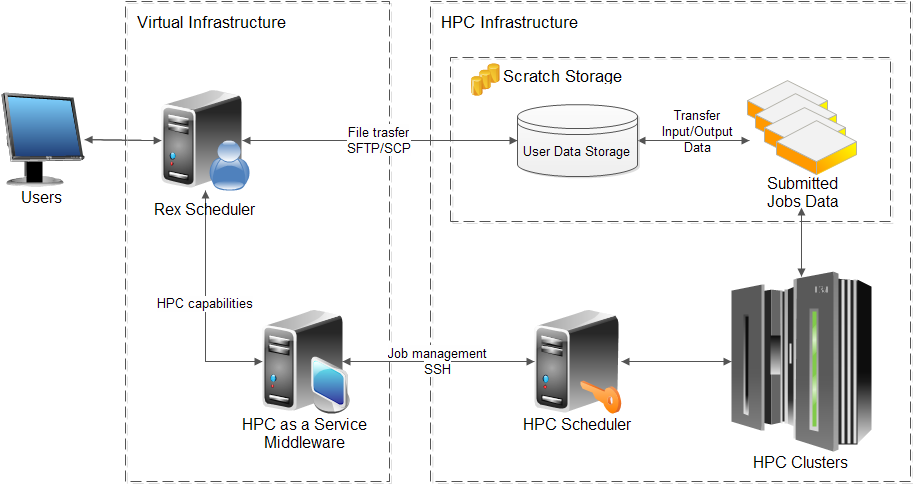
\includegraphics[width=0.8\textwidth]{Figures/haas.png}
	\caption{HPC-as-a-Service / HaaS \cite{uG7wIvjQiIli6kO9}}
	\label{fig:haas}
\end{figure}

\newpage
\section{Technické zázemí HEAppE Middleware}
Velký důraz je v tomto projektu kladen na multiplatformní využití a nezávislost použitého hardwaru. Tento aplikační framework je postaven na technologii .NET Core, poskytuje REST API a při nasazování je využívána kontejnerizační technologie Docker. Komunikace s plánovačem výpočetního uzlu probíhá prostřednictvím protokolu SSH, uživatel je autentizován jedním z uložených servisních účtů metodou RSA.

V současnosti tento framework zajišťuje komunikaci s plánovači PBS a Slurm. Podporuje autentizaci prostřednictvím SSH Agenta a je zajištěna podpora OpenID and OpenStack autentizace pro přístup k HEAppE Middleware API.

\subsection{Konfigurace HEAppE Middleware}
HEAppE je možné před spuštěním konfigurovat. V první řadě je sestaveno konfigurační schéma (docker-compose) pro službu Docker, na které middleware běží. Do této konfigurace mimo obraz HEAppE Middleware jsou zaneseny všechny podpůrné služby, jako je například MS SQL Server nebo SSH Agent. V návaznosti je přidána konfigurace samotné aplikace (AppConfig), která primárně specifikuje spojení s databází, port middleware API a další. Nedílnou součástí konfigurace je i počáteční stav dat uložených v databázi (seed), který si každý uživatel může specifikovat.

\subsection{REST API}
REST API je standardizované aplikační rozhraní využívající protokol HTTP. Služba poskytující toto API vystavuje tzv. endpointy a specifikaci pro práci s nimi. V případě HEAppE Middleware se jedná o url adresy se specifikací JSON struktury dat, které systém na vstupu očekává. Z praktického hlediska může jít např. o komunikační bod pro vytvoření specifikace úlohy, na vstupu se očekává JSON struktura popisující úlohu a specifický řetězec, který uživatel obdrží po autentizaci na jiném endpointu.

\subsection{Protokol SSH a metoda šifrování RSA}
Jak už bylo popsáno výše, HEAppE Middleware ke komunikaci s HPC clustery využívá protokolu SSH. Koncový uživatel je od této komunikace odstíněn a komunikuje pouze s vrstvou REST API. Při navazování spojení SSH je také odesílán soukromý klíč jednoho z nastavených servisních účtů v HEAppE Middleware, ten je následně porovnán s veřejným klíčem uloženým na HPC clusteru. Tato komunikace uživateli zaručuje bezpečnost pro práci, hlavní výhodou asymetrického RSA šifrování je vysoká složitost pro dešifrování, metoda je založena na prvočíselném rozkladu a je v současné chvíli prakticky neprolomitelná.

\subsection{Kontejnerizace a Docker}
Při nasazování systému je využívána technologie Docker. Ta umožňuje nakonfigurovat systém a pak už jen HEAppE Middleware sestavit na libovolném serveru. Docker automaticky stáhne požadované obrazy (image) a spustí systém. Výhoda je v přenositelnosti specifikace na jiné servery, kontejner je pak oddělen od ostatních, je možné specificky nastavit jeho komunikační rozhraní dle potřeb uživatele.

\subsection{Plánovače PBS a Slurm}
HEAppE Middleware v současnoti podporuje plánovače PBS a Slurm, tyto plánovače jsou hojně využívány v superpočítačových centrech po celém světě. Jedním z cílů HEAppE Middleware je platformí nezávislost, komunikační rozhraní jednotlivých plánovačů je však rozdílné a musí se k nim přistupovat individuálně. Koncový uživatel je však od této skutečnosti odstíněn a může tedy pracovat stále stejně, bez nutnosti znalosti dalšího systému. Na pozadí to řeší samotný middleware.


\section{Abstrakce HPC úlohy}
HEAppE Middleware poskytuje uživately určitou míru abstrakce nad skutečnou specifikací HPC úlohy. Úloha je v HEAppE nazvána jako Job. Job obsahuje obecné informace a nastavení, příkladem může být maximální doba běhu úlohy, zvolený cluster, maximální doba čekání na spuštění úlohy, definice proměnných využívaných při běhu programu. Každý z takto specifikovaných Jobů obsahuje minimálně jeden Task, tedy samostatnou specifikaci spouštěné úlohy na clusteru. Těchto tasků je možné definovat více, může u nich být specifikovaná návaznost na ostatní úlohy. Specifikace Tasku především obsahuje požadavky na využití jader, časový limit pro zpracování úlohy a další specifické parametry pro běh programu.

Tasky je možné spouštět jen z již vytvořených šablon, kde je definováno, jaký program se má na clusteru spouštět nebo jaké argumenty program má. Argumenty programu musí uživatel uvést vždy u specifikace úlohy (tasku).

Prostřednictvím HEAppE Middleware si uživatel definuje Job s Tasky, tento job pak může spustit a kontrolovat jeho stav. V průběhu zpracovávání je možné kdykoli úlohu zrušit. HEAppE uživateli poskytuje možnost kompletně úlohu spravovat, a to bez nutnosti znát principy komunikace s plánovačem HPC clusteru.

Příklad struktury příkazu ke spuštění úlohy na HPC clusteru, který plně nahrazuje jeden HEAppE RestAPI endpoint:

\begin{lstlisting}[language=bash,caption={Struktura příkazu qsub \cite{iR8VZfeCCZ757gs1}}]
qsub -q <queue> -w e -N <job_name> -l h_vmem=<memory> -l h_rt=<time> -l s_rt=<time> -pe smp <num_slots> -o <outputlogfile> -e <errorlogfile> <pathtoScript> <arg1> <arg2>
\end{lstlisting}

\section{Uživatelské a servisní účty}
HEAppE Middleware mapuje virtuální HEAppE uživatelské účty na skutečné clusterové účty (servisní). Správce HEAppE instance je oprávněn k vytváření „virtuálních“ uživatelských účtů. Uživatel se autentizuje prostřednictvím svého loginu a hesla, OpenID nebo OpenStack v HEAppE. Následně obdrží vygenerovaný klíč (alfanumerický hash) s časově omezenou platností. Při volání dalších HEAppE RestAPI endpointů tento hash využívá. Při konečné komunikaci superpočítačovým clusterem HEAppE využívá jeden z uložených servisních účtů. Tyto účty jsou schváleny superpočítačovým centrem a správce HEAppE instance stojí za spouštěnými úlohami. 

HEAppE Middleware tyto clusterové (servisní) účty střídá, aby nedošlo k zablokování ze strany superpočítačového centra. Systém bez rotace využívaných účtů by mohl nést znaky DDOS/DOS útoku a účty by mohly být preventivně zablokovány.vvv

Z výše uvedeného textu je zřejmé, že uživatelé spouštějící úlohy prostřednictvím HEAppE Middleware mohou ve skutečnosti využívat jeden servisní clusterový účet. HEAppE řeší přístupy uživatelů k jejich datům na výpočetním clusteru.

Tento popsaný princip rozšiřuje předešlou úvahu o využívání osobních clusterových účtech. Kde platí, že 1 ověřený uživatel komunikuje se superpočítačem (s jeho plánovačem) pomocí svého osobního clusterového účtu.

\section{Zajímavé funkcionality HEAppE Middleware}
\subsection{JobArrays}
K úlohám definovaným prostřednictvím HEAppE je možné přidat specifikaci pro opakování spouštění úlohy. Tato funkcionalita je nazvána jako JobArrays, teminologie vychází z funkce plánovače. Uživatel specifikuje iterace dané úlohy a plánovač pak úlohu spouští v cyklu. Praktické využití této funkce je například u renderování scén a vykreslování grafiky.
Příklad dormátu pro definování JobArrays:


\begin{lstlisting}[language=bash,caption={Struktura definice JobArrays}]
                            <start_index>-<end_index>:<step>
\end{lstlisting}

\subsection{Závislosti úloh}
U jednotlivých úloh, které jsou součástí struktury Job, je možné na sebe navazovat. Uživatel může jednoduše definovat závislosti úloh. Prakticky se jedná o podmíněné spouštění dalších navázaných úloh až po úspěšném vykonání úlohy předešlé. Omezuje se tímto možné plýtvání prostředky a výpočetním časem, které by mohlo nastat při selhání jedné z úloh, na jejímž výstupu závisí úloha další.

HEAppE ale musí řešit kontrolu těchto závislostí, aby nedošlo ke kruhové/cirkulární závislosti. Zjednodušeně je tento problém možné specifikovat jako problém s nekonečným čekáním. Na straně výpočetního clusteru by mohl nastat tzv. Deadlock. Jedná se o uváznutí systému při vzájemném čekání. Na superpočítači se tento problém řeší kontrolou specifikace úloh a také detekcí kruhové závislosti v grafu. HEAppE cirkulární závislost kontroluje také, aby se celý proces urychlil a nedocházelo by k chybám na straně výpočetního clusteru. Na následujícím snímku se nachází znázornění typického uváznutí – cirkulární závislosti procesů (P1, P2) a prostředků (R1, R2). Závislost je znázorněna šipkou.


\begin{figure}
	\centering
	
\includegraphics[width=0.4\textwidth]{Figures/Process_deadlock.png}
	\caption{Cirkulární závislost \cite{OvBwjLleECKerU0E}}
	\label{fig:cirkularni-zavislost}
\end{figure}

\newpage
\subsection{Extrémně dlouhé úlohy}
Každý uzel superpočítačového clusteru má definován horní interval pro dobu vykonávání uživatelských úloh (Walltime Limit). Systém ukončí každou úlohu, pokud přesáhne časový limit pro vykonávání úlohy. Existují ale uživatelé, jejichž programy vyžadují extrémně dlouhý čas pro dokončení, který překračuje již zmíněný limit na uzlu superpočítačového clusteru. I na tento problém HEAppE Middleware pamatuje. Při definování úlohy je možné nastavit přepínač pro vykonávání v režimu „ExtraLong“. V tomto případě HEAppE logicky rozdělí úlohu na více podúloh se závislostmi na postupném zpracování. Rozdělení pobíhá podle uživatelem uvedeného časového limitu a limitu pro zpracovávání na požadovaném uzlu superpočítače. Výhodou je to, že je uživatel odstíněn od manuálního rozdělování úlohy na podúlohy. Dále je takto upravená specifikace úlohy předána plánovači na superpočítači a ten se již stará o vykonání úlohy.

\hfill \break
\begin{figure}[h]
	\centering
	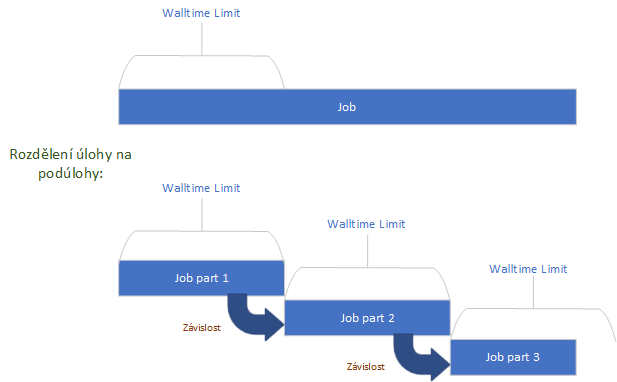
\includegraphics[width=0.8\textwidth]{Figures/job-decompose.png}
	\caption{Rozdělení extrémně dlouhé úlohy }
	\label{fig:rozdeleni-extra-long}
\end{figure}